\section{Schlauchbeutelmaschine}
Mit diesem Beispiel kann man die bestehende Architektur durch eine weitere Maschine ergänzen. Es ist problemlos möglich
auch Weitere oder andere Maschinen oder gar Module einer Maschine einzurichten. Allerdings soll mit diesem Beispiel die
allgemeine Vorgehensweise erklärt werden und dieses Beispiel veranschaulicht dies.

In Abbildung~\ref{fig:siegelmaschinen_vffs} auf Seite~\pageref{fig:siegelmaschinen_vffs} ist der schematische Aufbau der
vertikalen Schlauchbeutelmaschine abgebildet.

\begin{figure}[h]
    \centering
    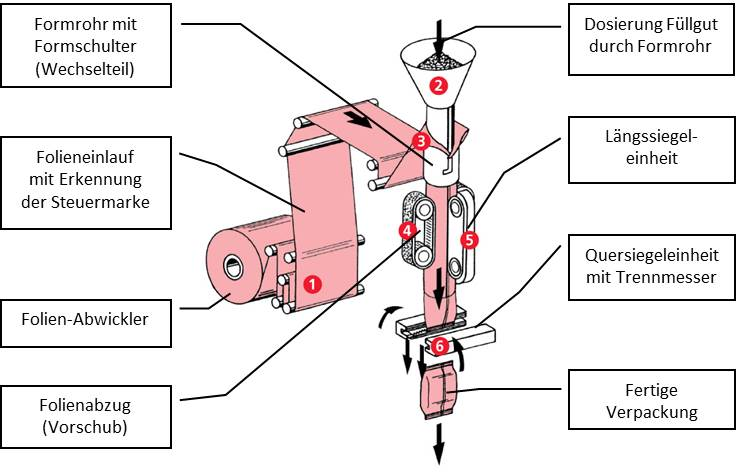
\includegraphics[scale=1]{images/kapitel_5/vffs.jpg}
    \caption{Aufbau einer vertikalen Schlauchbeutelmaschine~\cite{online_grundlagen_boschkwe}}
    \label{fig:siegelmaschinen_vffs}
\end{figure}

Dort ist gut zu sehen, dass im oberen Bereich der Abbildung, unter der Nummer 2, dass zu befüllende Produkt einlegt
wird. Dies fällt dann durch das Rohr mit der Nummer 3. Die Folie umschließt das Produkt anschließend und diese wird mit
den Siegelbacken (Nummer 5) versiegelt. Bei Nummer 6 trennt ein \textit{Trennmesser} den befüllten Beutel von der
Endlosfolie ab und so kann der befüllte Beutel weiterverarbeitet werden.

Die wichtigsten Einstellparameter der Maschine betreffen die Siegelung des Beutels. Da zahlreiche Folienarten von
verschiedenen Anbietern existieren ist es nicht immer einfach, die Folie richtig und korrekt zu versiegeln.

Die \textit{Siegelnahtfestigkeit} gibt an, welche Kraft notwendig ist, um die verschlossene Siegelnaht wieder zu öffnen.
Dies ist insbesondere dann Wichtig, wenn es sich bei dem verpackten Produkt um ein Endkunden-Produkt handelt. Der Käufer
sollte die Verpackung unter normalem Kraftaufwand öffnen können, damit er an das Produkt gelangen kann.

Allerdings darf die Siegelnaht nicht zu schwach sein, da sonst Luft oder andere Gase in die Verpackung eindringen
könnten. Für die vertikalen Schlauchbeutelmaschine ist es entscheidend die richtige Siegelnahtfestigkeit zu erzeugen.

Zur Erzeugung einer Siegelnaht sind Daten zur \textit{Siegeltemperatur}, \textit{Siegelzeit} und \textit{Folienart}
interessant. Bei der Folie spielt der Aufbau der Folie (anzahl der Lagen und genutzte Materialien) eine Rolle.

Der genaue Aufbau von Folien wird von den entsprechenden Herstellern oft geheim gehalten und man muss ihn entweder
händisch ermitteln oder auf Erfahrungen von Mitarbeitern zurückgreifen.

Aus diversen Tests kann man anhand der eingestellten Parameter für Siegeltemperatur und Siegelzeit und der genutzten
Folie die Siegelnahtfestigkeiten ableiten, indem man den Kraftaufwand zum öffnen der Siegelnaht misst.

Für das weitere Beispiel ist es nun interessant die Siegelnahtfestigkeit aus einem neuronalen Netz zu ermitteln, sofern
die Zusammensetzung der Folie sowie die Siegeltermperatur und Siegelzeit feststeht.

Ein weiteres Beispiel könnte sein, die Siegelnahtfestigkeit und genutzte Folie vorzugeben und das neuronale Netz
ermitteln zu lassen, welche Temperatur und welche Zeit für das Siegeln eingeplant werden muss. Dieses Beispiel wird
aktuell aber nicht weiter verfolgt.

\subsection{Daten zusammenstellen}
Um an Testdaten für das Aufbauen eines neuronalen Netzes für diesen Maschinentyp zu kommen, sind zahlreiche
zeitintensive Tests und Versuche notwendig.

Für die Versuche muss man verschiedene Temperaturen mit verschiedenen Siegelzeiten mit verschiedenen Folien kreuzen, was
einen enormen Zeitaufwand bedeutet.

Durch eine Zugprüfmaschine kann man anschließend die Schälfestigkeit bestimmt -- die Kraft, die bei einer schälenden
Beanspruchung aufgewendet werden muss -- um eine Naht zu öffnen. Die Prüflinge sollten dabei eine Breite von 15mm und
eine Länge 40mm aufweisen.

Herr Felix Kruppa von der Robert Bosch GmbH hat während seiner Dissertation einen Siegelteststand aufgebaut, welcher
verschiedene Siegelnähte mit unterschiedlichen Siegelzeiten und "~temperaturen erzeugen kann.

Für den Aufbau seines Teststandes durchlief er zahlreiche Tests, welche er mit einem Protokoll dokumentierte. Diese
Daten können für die Erstellung des neuronalen Netzes fungieren, da er ebenfalls die resultierende Siegelnahtfestigkeit
ermittelte und in seiner Dokumentation festhielt.

In Abbildung~\ref{fig:siegelmaschinen_vffs_simulator} auf Seite~\pageref{fig:siegelmaschinen_vffs_simulator} ist der
aufgebaute Siegelteststand von Herrn Felix Kruppa mit Beschriftungen zu sehen.

\begin{figure}[h]
    \centering
    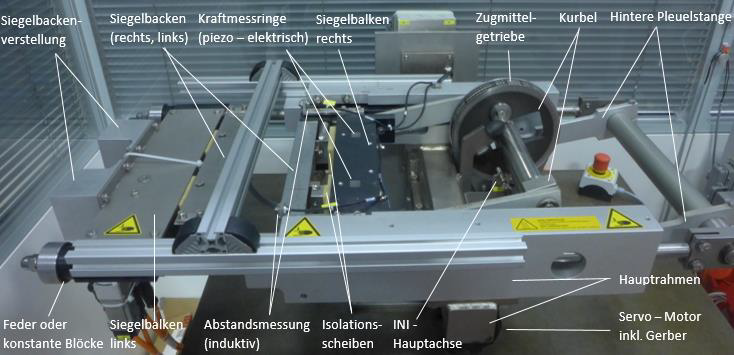
\includegraphics[width=\textwidth]{images/kapitel_5/vffs_simulator.png}
    \caption{Aufbau des Siegelteststandes}
    \label{fig:siegelmaschinen_vffs_simulator}
\end{figure}

Die kombinierten Daten aus den Testdurchläufen von Herrn Kruppa sind im Anhang~\ref{sec:schlauchbeutelmaschine}
auf Seite~\pageref{sec:schlauchbeutelmaschine} zu sehen und man kann diese direkt für das Trainieren des neuronalen
Netzes in der Cloud oder auch offline nutzen.

\subsection{Neuronales Netz trainieren}
Mit Hilfe der zusammengestellten Testdaten kann man nun das neuronale Netz trainieren. Das Training funktioniert in
gleicher Weise wie auch in Kapitel~\ref{subsub:modeler_flow} ab Seite~\pageref{subsub:modeler_flow} mit dem Modeler
Flow in der IBM Cloud.

Dazu werden die Testdaten in den Watson Studio Service hochgeladen und anschließend mit einem Data Refinery Flow in eine
CSV-Datei umgewandelt. Der Machine Learning Service der IBM Cloud kann aktuell lediglich mit CSV-Dateien zum Trainieren
von neuronalen Netzen umgehen.

Auch kann man die Datei schon auf dem Entwicklungsrechner in eine CSV-Datei konvertieren um sich die Konvertierung im
Service zu sparen. So muss man keinen neuer Flow für die Data Refinery anlegen. Es spielt keine Rolle wo man die Datei
konvertiert.

Anschließend muss man einen neuen Modeler Flow anlegen und diesen genau gleich dem Flow in
Abbildung~\ref{fig:umsetzung_model_flow} auf Seite~\pageref{fig:umsetzung_model_flow} aufbauen.

In diesem Fall ändern sich aber die Parameter für die Eingabe"~ und Ausgabeparameter wie in
Tabelle~\ref{tab:targets_inputs_siegeln} auf Seite~\pageref{tab:targets_inputs_siegeln} zu sehen.

\begin{table}[h]
    \centering
    \begin{tabular}{|c|c|}
        \hline
        \textbf{Targets} & \textbf{Inputs}\\
        \hline
        \hline
        Mittelwert & Eindringverhalten\\
        \hline
        & Temperatur\\
        \hline
        & Vorwärmphase\\
        \hline
        & Eindringphase\\
        \hline
        & Siegelphase\\
        \hline
        & End-Siegel-Position\\
        \hline
    \end{tabular}
    \caption{Variablen für die Targets und die Inputs der Schlauchbeutelmaschine}
    \label{tab:targets_inputs_siegeln}
\end{table}

Nach erfolgreicher Konfiguration der einzelnen Module kann man das neuronale Netz trainieren lassen um das Modell zu
erhalten. Diese Modell kann man dann im Weiteren in einem Deployment zur Verfügung stellen.

\subsection{Deployment erstellen}
Um das Deployment für das trainierte Modell zu erstellen, muss man das Modell im Modeler Flow mit der rechten Maustaste
auswählen und \enquote{Save branch as a model} auswählen. Dies speichert das trainierte Modell als eigenständiges Modell
im Watson Studio ab.

Dies kann man nun über das Watson Studio Dashboard auswählen und über den Reiter \texttt{Deployments} auf alle
Webservices des einen Modells zugreifen. Dort sind aktuell aber noch keine sichtbar.

Über die Schaltfläche \texttt{Add Deployment} legt man ein neues an. Dies geschieht genau wie in
Kapitel~\ref{subsec:deployment_erstellen} ab Seite~\pageref{subsec:deployment_erstellen} beschrieben.

Nach der Eingabe eines Namens und der Speicherung des Deployments erscheint es in der vorher leeren Liste. Damit das das
trainierte Modell in einem Webservice zur Verfügung getsellt.

In der Abbildung~\ref{fig:siegelmaschinen_deployment} auf Seite~\pageref{fig:siegelmaschinen_deployment} ist die
komplette Konfiguration des Deployments für den Webservice ersichtlich.

\begin{figure}[h]
    \centering
    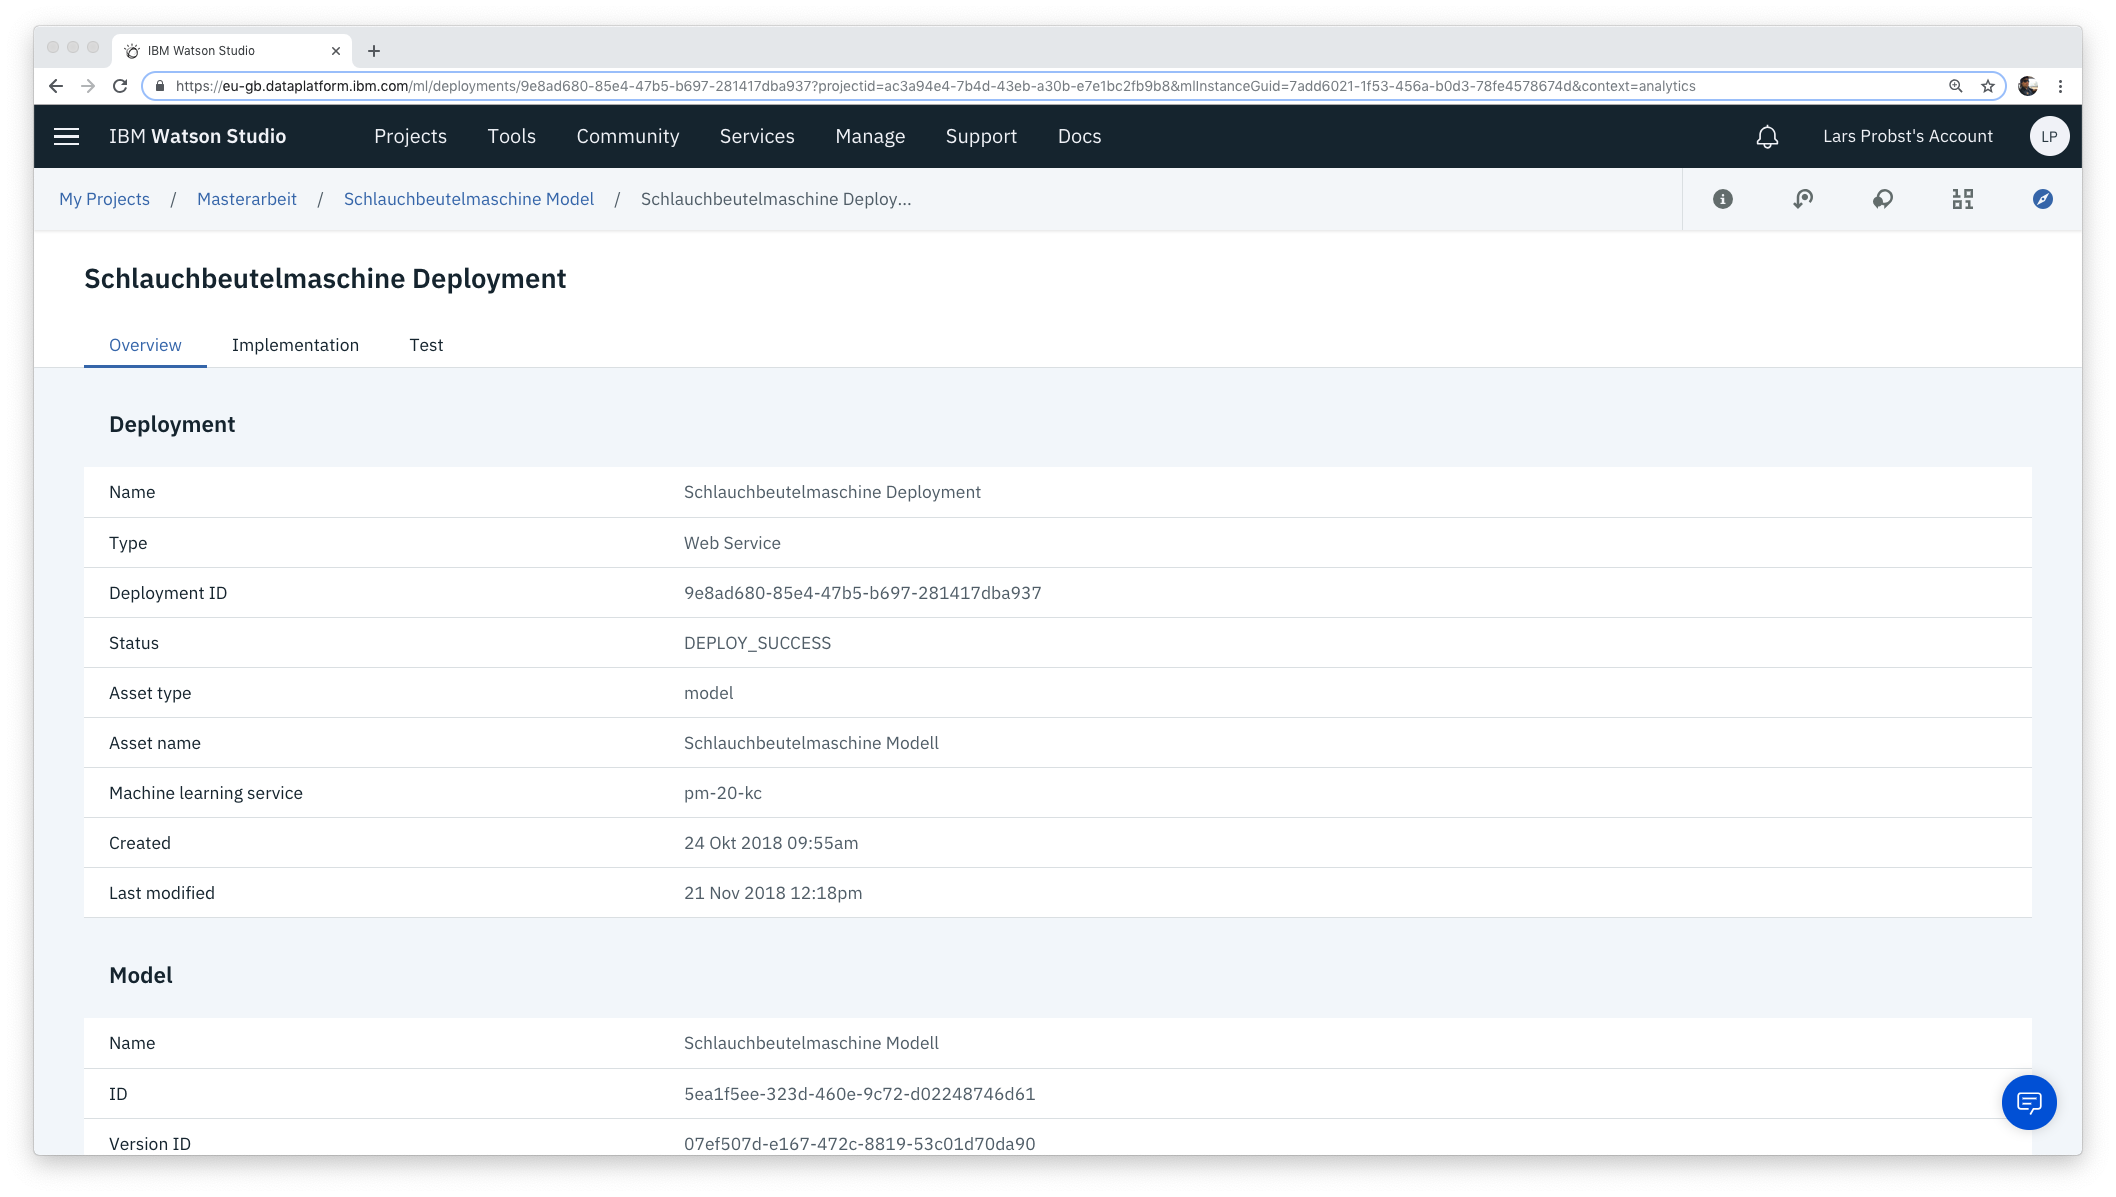
\includegraphics[width=\textwidth]{images/kapitel_5/vffs_deployment.png}
    \caption{Deployment der Schlauchbeutelmaschine}
    \label{fig:siegelmaschinen_deployment}
\end{figure}

Nun kann man in einem weiteren Schritt den API Connect Service um diesen Endpunkt erweitern, um auch Vorhersagen von
diesem neuronalen Netz zu beziehen um die Siegelnahtfestigkeit zu ermitteln.

\subsection{API Connect erweitern}
Der API Connect Service fungiert als Knotenpunkt zwischen Frontend und den möglichen Vorhersage-Services. Damit das
Frontend auf neue Services vereinfacht zugreifen kann, muss man hier einen neuen Endpunkt anlegen. Dies kann man
entweder über die Erweiterung der JSON-Konfiguration oder über den grafischen Editor machen.

Der einfachere Weg ist die Anpassung der Endpunkt über den grafischen Editor. Damit man den neuen Service auch über den
API Service nutzen kann, muss man im Reiter \texttt{Gestalten} in der Konfiguration \texttt{Pfade} einen neuen anlegen.

Diesen kann man beliebig benamen. Ein Beispiel hierfür ist \textit{predict-seal}. Darüber hinaus muss der Pfad eine
Operation besitzen. Diese muss, genau wie alle anderen Operationen der anderen Pfade, \textit{POST} sein, damit das
Frontend Daten an den Endpunkt schicken kann.

Da der neue Pfad angelegt ist, kann man die Konfiguration speichern und in den Reiter \texttt{Assemblieren} wechseln.
Der \textit{Switch} für die Verzweigung je nach gewünschtem Pfad muss man um den gerade eingerichteten neuen Pfad
erweitern. Somit beinhaltet die Switch-Operation drei Verzweigungen.

Der Inhalt für den neuen Pfad kann man direkt vom Pfad \textit{predict-watson} übernehmen und lediglich im
\textit{Get Prediction} Modul definierte URL für den Webservice anpassen.

Die Abbildung~\ref{fig:siegelmaschinen_apiconnect} auf Seite~\pageref{fig:siegelmaschinen_apiconnect} veranschaulicht
den angepassten Modeler Flow um den neuen Endpunkt.

\begin{figure}[h]
    \centering
    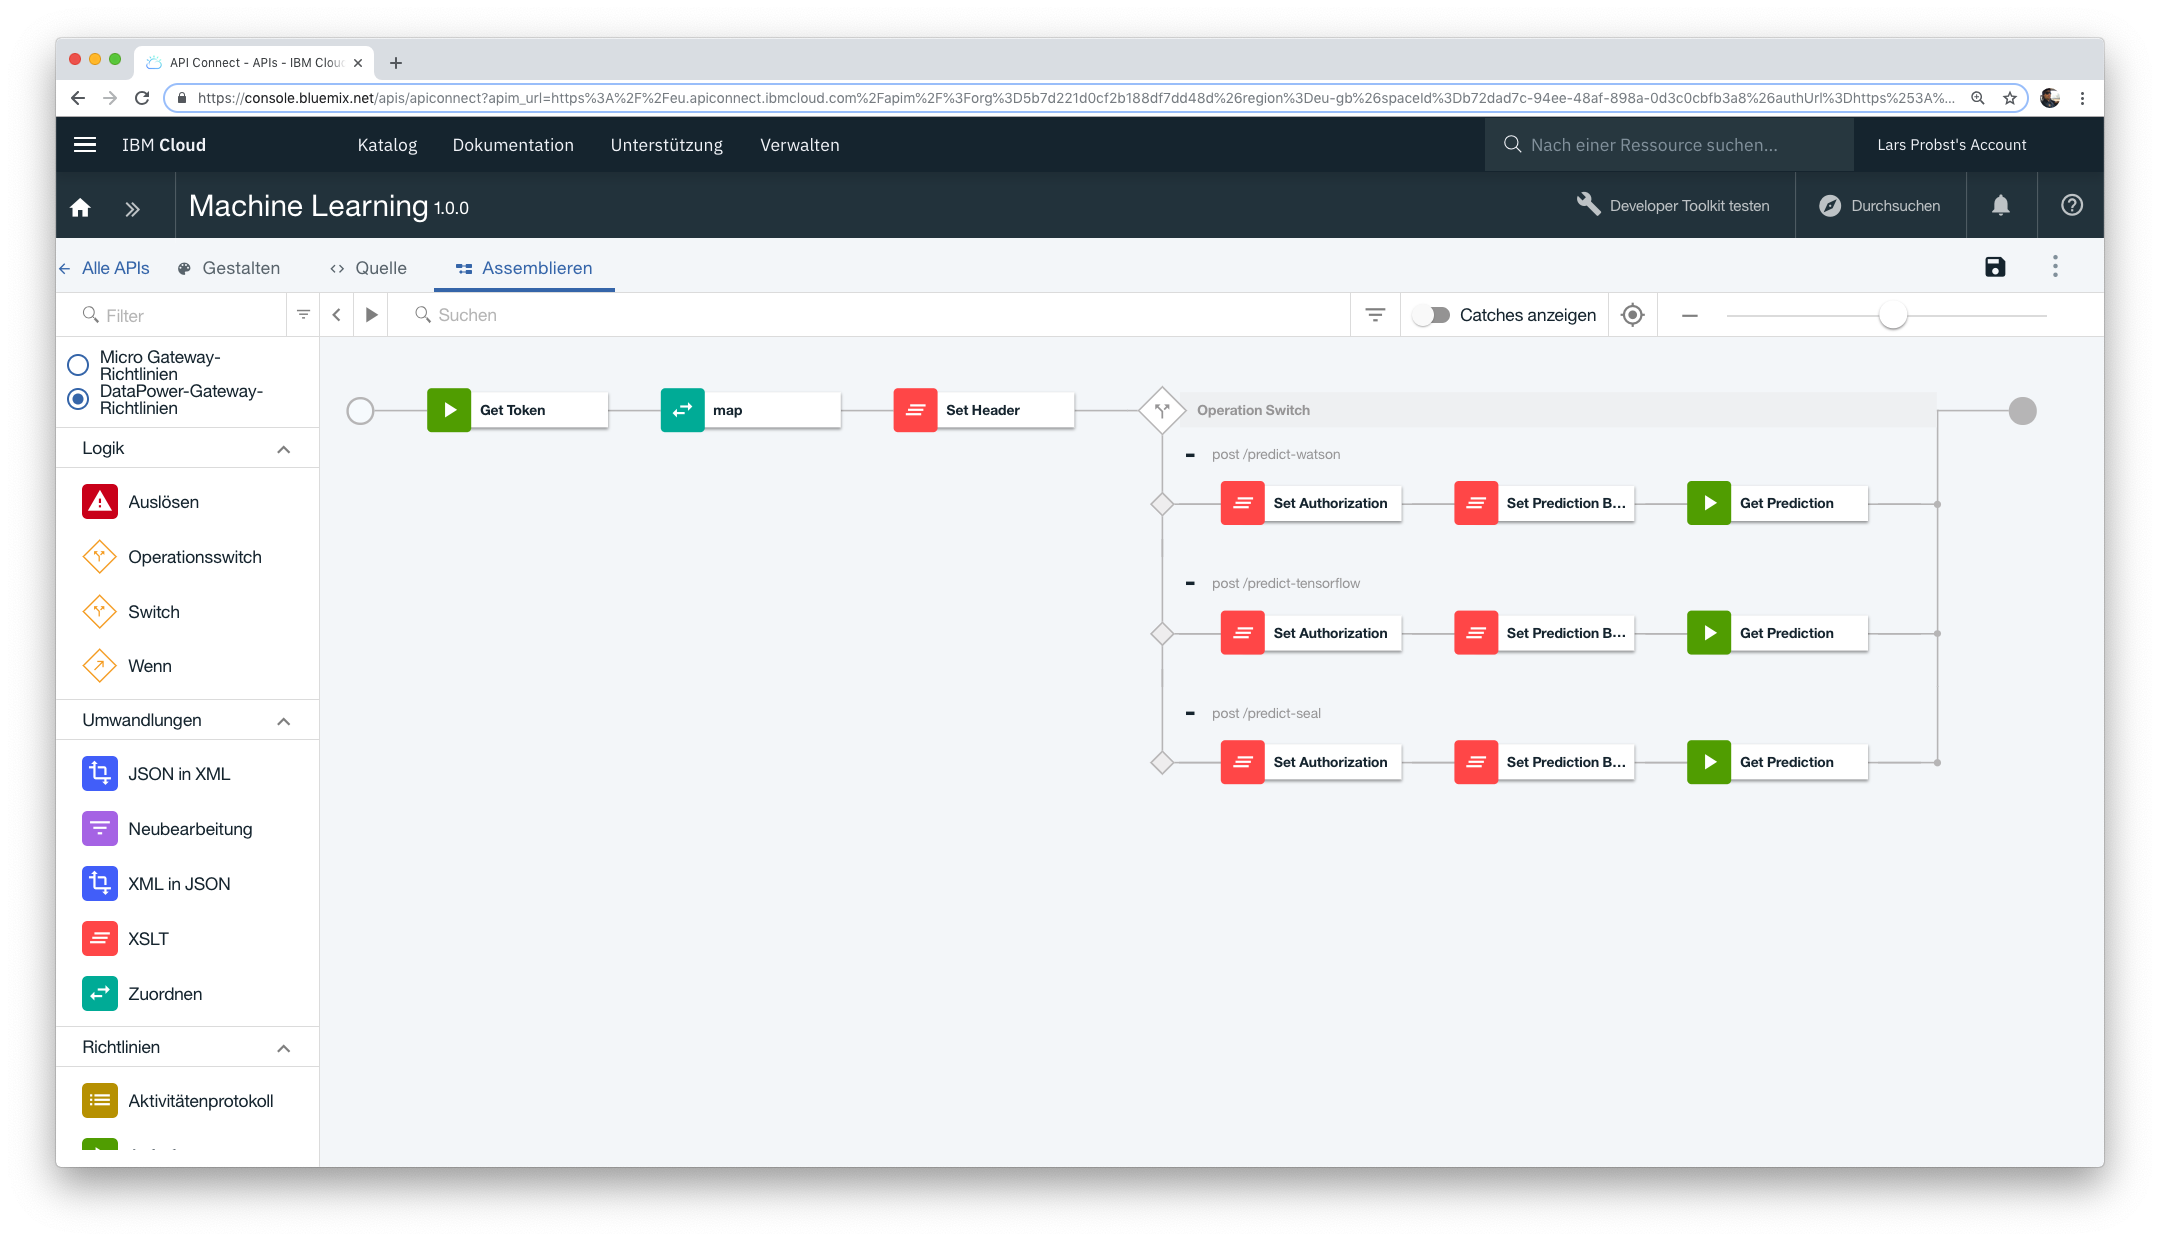
\includegraphics[width=\textwidth]{images/kapitel_5/vffs_apiconnect.png}
    \caption{Angepasster API Connect Service}
    \label{fig:siegelmaschinen_apiconnect}
\end{figure}

Damit ist der API Connect Service fertig eingerichtet und man kann den neuen Endpunkt zum Beispiel vom Frontend aus
abrufen. Auch ist es Möglich den Aufruf mittels Postman zu überprüfen. Ein Test sollte die Funktionsweiße des Endpunktes
sicherstellen.

\subsection{Frontend erweitern}
Im letzten Schritt der Adaptierung der Architektur auf eine neue Maschine oder auf ein neues Modul muss man das Frontend
um die gewünschten Eingaben der Parameter erweitern, damit das Frontend die Vorhersage auf dem Webservice starten und
das Ergebnis darstellen kann.

Dafür kann man eine neue Angular-Komponente anlegen und diese dann mit dem gewünschten neuen Design versehen. Das
Anlegen einer Komponente in Angular geschieht am Einfachsten über ein Kommando der Angular-CLI.

\begin{lstlisting}[caption=Erstellen einer neuen Komponente, label=ls:schlauchbeutelmaschine_component]
    ng generate component name
\end{lstlisting}

Der Parameter \textit{Name} dient als Platzhalter und man muss ihn mit einem Namen für die Komponente ersetzen. Dieser
Name darf durch keine andere Komponente vergeben sein. Die neue Komponente erscheint als Unterordner im Ordner
\texttt{app}.

Die neue Komponente besteht aus den vier Dateien \textit{*.component.css} für die Definition von CSS-Eigenschaften,
\textit{*.component.html} zur Konfiguration der Darstellung, \textit{*.component.spec.ts} für das Schreiben von Tests
und \textit{*.component.ts} für die eigentliche Logik.

Der Inhalt der vier Dateien kann man aus der Komponente für die Waage im Ordner \texttt{/app/scales} kopieren und
anschließend Stück für Stück anpassen.

In der HTML-Datei muss man das Design auf die neuen Eingabefelder abändern. Dies ist Wichtig, da andere Parameter für
den Endpunkt notwendig sind.

In der TS-Datei, in der die Logik der Komponente definiert ist, muss man den REST-Endpunkt auf den neuen Namen abändern
und die übergebenen Parameter anpassen, damit die Vorhersage auch funktionieren kann.

Auch ist entscheidend, dass man die Abfrage zu leeren Felder auf die richtige Benamung und die definition von
zufälligen Eingabeparameter auf logische Werte anpasst. So ist es für einen Endnutzer möglich schnell einen Test über
das Frontend zu starten.

Die CSS-Datei sowie die SPEC-Datei bedürfen keiner zwingenden Änderung, da sie für die Funktionsfähigkeit der Abfrage an
das Backend keine Rolle spielen. Allerdings sollte man zu einem späteren Zeitpunkt den Test für die Komponente
berichtigen.

\subsection{Abschluss}
An diesem Punkt ist die Adaption der erstellen Architektur auf die Siegelmaschine abgeschlossen und man kann damit
beginnen, neue Vorhersagen des neuen Webservices durch das Frontend zu beziehen. Die Ergebnisse werden anschließend
ebenfalls auf dem Frontend angezeigt.

Für alle weiteren Anpassungen oder Erweiterungen der Architektur muss man lediglich diese fünf relativ einfachen
Schritte wiederholen und um die neuen Einstellungen anpassen.

Damit ist gezeigt, dass die gebaute Architektur so modular ist, um sie problemlos zu erweitern und neue Funktionen
darin einzubauen. Dies galt es als Teilaufgabe in der Arbeit zu zeigen und beweisen.